\documentclass[12pt]{exam}
\usepackage[utf8]{inputenc}
\usepackage[T1]{fontenc}
\usepackage{wrapfig}
\usepackage{amsmath}
\usepackage{amssymb}
\usepackage{hyperref}
\usepackage{graphicx}
\usepackage{fontawesome}
\usepackage[norsk]{babel}
\usepackage{tikz}
\usetikzlibrary{shapes}
\usepackage{tkz-euclide}
\usepackage{float}
\usepackage{wrapfig}
\usepackage{pgfplots}
\pgfplotsset{compat=1.11}
\usetikzlibrary{decorations.pathreplacing}
\definecolor{rvwvcq}{rgb}{0.08235294117647059,0.396078431372549,0.7529411764705882}
\definecolor{wrwrwr}{rgb}{0.3803921568627451,0.3803921568627451,0.3803921568627451}
\begin{document}

\pagestyle{headandfoot}
\runningheadrule
\firstpageheader{}{}{}
\firstpagefooter{}{}{}
\runningheader{Eksamenskurs i matematikk for ungdomskolen 2018}{}{\includegraphics[width=0.2\textwidth]{./img/logo.jpg}}
\runningfooter{}{}{}



{  \centering

	{\scshape\Huge Eksamenskurs i matematikk \par}
	\vspace{1cm}
	{\Large Ungdomskolen \today \par}
	\vspace{1.5cm}
        \begin{center}
          { \large
          \begin{tabular}{c | c}
            Tid & Hva \\ \hline
            16:15-17:30 & Geogebra og geometri\\ \hline
            17:30-17:45 & Pause \\\hline
            17:45-19:00 & Geogebra og geometri\\\hline
          \end{tabular}
          }
          \vspace{1.5cm}
          \begin{figure}[h!]
            \centering
            \includegraphics[scale = 0.7]{./img/forside.png}                      
          \end{figure}

        \end{center}

}

\newpage

\qformat{\bf \large \underline{Oppgave  \thequestion} \hfill}

\begin{questions}
  \section*{Geometri}
  % http://www.math-exercises.com/stereometry/volume-and-surface-area-of-solids
  % Oppgave
\begin{minipage}{0.7\linewidth}
  \question Finn volumet og overflaten til en kube der en side har overflate $40cm^2$.
\end{minipage}
\hspace{1cm}
\begin{minipage}{0.2\linewidth}
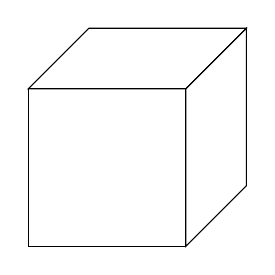
\begin{tikzpicture}[scale = 2]
\pgfmathsetmacro{\cubex}{1}
\pgfmathsetmacro{\cubey}{1}
\pgfmathsetmacro{\cubez}{1}
\draw (0,0,0) -- ++(-\cubex,0,0) -- ++(0,-\cubey,0) -- ++(\cubex,0,0) -- cycle;
\draw (0,0,0) -- ++(0,0,-\cubez) -- ++(0,-\cubey,0) -- ++(0,0,\cubez) -- cycle;
\draw (0,0,0) -- ++(-\cubex,0,0) -- ++(0,0,-\cubez) -- ++(\cubex,0,0) -- cycle;
\end{tikzpicture}
\end{minipage}
%% V = 253 cm3, OV = 240 cm2
\question

\begin{minipage}{0.7\linewidth}
En sylindrisk vase har en høyde på $28cm$ og en intern diameter på $1.1dm$.
Hvor mange liter vann skal til for å fylle vasen dersom tykkelsen på bunnen er $1.5cm$.
\end{minipage}%
\hspace{1cm}
\begin{minipage}{0.2\linewidth}
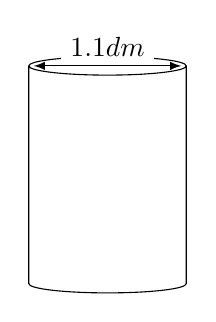
\begin{tikzpicture}[>=latex,shorten >=2pt,shorten <=2pt,shape aspect=1]
\node (A) [cylinder, shape border rotate=90, draw,minimum height=3cm,minimum width=2cm]{};
\draw [<->] (A.before top) -- (A.after top) node [midway, above,fill=white] {$1.1dm$};
\end{tikzpicture}
\end{minipage}
%% V = 2.52 l

% Oppgave
\question
Ett sylinder med diameter $1.8m$ og inneholder $2000 l$ vann. Hvor høyt står vannet i sylinder et?
%% 78.63 cm


% Oppgave
\question
\begin{minipage}{0.7\linewidth}
Finn volumet og overflaten av kjegla der $h=46mm$ og $r =2.3dm$.
\end{minipage}
\begin{minipage}{0.3\linewidth}
  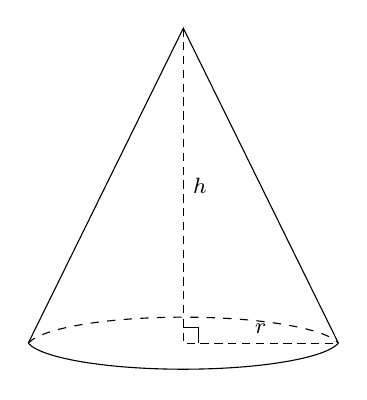
\begin{tikzpicture}
    \draw[dashed] (0,0) arc (170:10:2cm and 0.4cm)coordinate[pos=0] (a);
    \draw (0,0) arc (-170:-10:2cm and 0.4cm)coordinate (b);
    \draw[densely dashed] ([yshift=4cm]$(a)!0.5!(b)$) -- node[right,font=\footnotesize] {$h$}coordinate[pos=0.95] (aa)($(a)!0.5!(b)$)
                            -- node[above,font=\footnotesize] {$r$}coordinate[pos=0.1] (bb) (b);
    \draw (aa) -| (bb);
    \draw (a) -- ([yshift=4cm]$(a)!0.5!(b)$) -- (b);
  \end{tikzpicture}
\end{minipage}
% V = 2,548.25 cm3, SA = 3,356.72 cm2

\question
En kjegle og ett sylinder har begge ett volum på $180cm^3$ og en høyde på 15cm. Hvilket legeme har størst overflate?
% Sylynderet  

% Oppgave
\question
\begin{minipage}{0.7\linewidth}  
En gassbeholder i formen av en kule har en diameter på $14m$. Hvor mange $m^3$ med gass får plass i beholderen?
\end{minipage}
\begin{minipage}{0.3\linewidth}
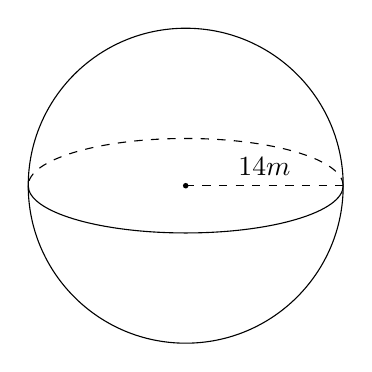
\begin{tikzpicture}
%  \shade[ball color = gray!40, opacity = 0.4] (0,0) circle (2cm);
  \draw (0,0) circle (2cm);
  \draw (-2,0) arc (180:360:2 and 0.6);
  \draw[dashed] (2,0) arc (0:180:2 and 0.6);
  \fill[fill=black] (0,0) circle (1pt);
  \draw[dashed] (0,0 ) -- node[above]{$14m$} (2,0);
\end{tikzpicture}
\end{minipage}
%% 1,436.8 m3
\newpage
% Oppgave
\question
$ $ \vspace{0.5cm}

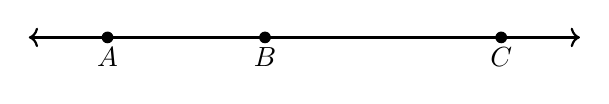
\begin{tikzpicture}
  \draw[thick,<->] (-1,0) -- (6,0);
  \tkzDefPoint(0,0){A}
  \tkzDefPoint(2,0){B}
  \tkzDefPoint(5,0){C}
  \tkzLabelPoint[below](A){$A$}
  \tkzLabelPoint[below](B){$B$}
  \tkzLabelPoint[below](C){$C$}
  \foreach \n in {A,B,C}
  \node at (\n)[circle,fill,inner sep=1.5pt]{};
\end{tikzpicture} $ $\\
Linja $AC$ er 23. Lengden av linja $AB$ er gitt ved $3x-46$ og lengden av linja $BC$ er $4x - 57$. Hvor lang er $AB$? 
\section*{Geogebra}
% Oppgave
\question 
Finn skjæringspunktet til linja $PH = 5+2x$ og linja $DQ = 4x - 17$. Bruk deretter Geogebra for å kontrollere svaret. 
% Oppgave
\question
Bruk Geogebra til å tegne punktene $A =(0,0), B=(0,3), C=(3,1)$ ved hjelp av {\em polygons}. Bruk så {\em Mesure} til å regne ut arealet av trekanten $ABC$.
% Oppgave  
  \question
  \begin{minipage}{0.5\linewidth}
  \begin{parts}
    \part Lag i Geogebra  kvadratet $ABCD$ der lengden av hver side er 5.\\
    \part Hva er arealet av det grå området?\\
    \part Hvor lang er linja $AC$?
    \part Bruk Geogebra til å finne  arealet og lengden $AC$.
  \end{parts}
\end{minipage}%
\begin{minipage}{0.5\linewidth}
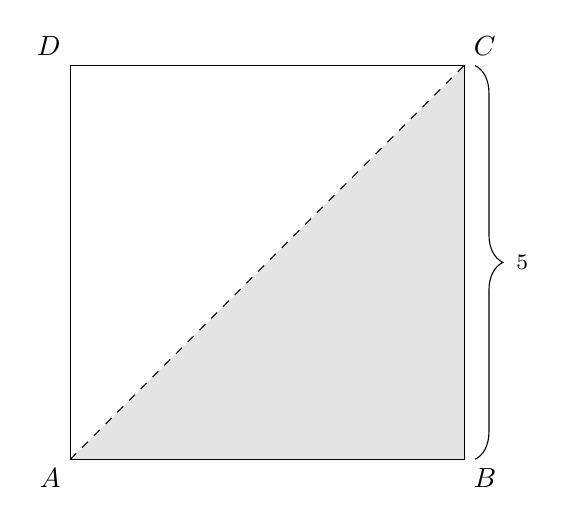
\begin{tikzpicture}
  \fill[fill=gray!20] (0,0) -- (5,5) -- (5,0);
  \draw (0,0) node[anchor=north east]{$A$} -- (5,0) node[anchor=north west]{$B$}-- (5,5) node[anchor=south west]{$C$}-- (0,5)node[anchor=south east]{$D$} -- cycle;
  \draw[dashed] (0,0) -- (5,5);

  \draw [decorate,decoration={brace,amplitude=10pt,mirror},xshift=4pt,yshift=0pt]
  (5,0) -- (5,5) node [black,midway,xshift=0.6cm]
  {\footnotesize 5};
\end{tikzpicture}
\end{minipage}%

%Oppgave
\question
 Tidligere lagde dere ett kvadrat i Geogebra ved å lage punkter og linjer. I denne oppgaven skal vi først lære en ny funksjon som på engelsk heter ''perpendicular line'' dette betyr på norsk en vinkelrett linje.\\
 Tegn ved hjelp av Geogebra en linje og et punkt i planet. Bruk ''perpedicular line'' til å tegne en linje som står vinkelrett på den linja du tegna og går igjennom punktet.
\newpage
 \question
 I denne oppgaven skal vi konstruere den vinkelrette linja ved hjelp av {\emph compass} som betyr passer på norsk. Dette gjøres som følger
 \begin{enumerate}
 \item Tegn en linje og to punkter på denne.
 \item Tegn to tilstrekkelig store sirkler som har lik radius med compass.
 \item Marker de to skjæringspunktene sirklene.
 \item Trekk så en linje mellom disse to skjæringspunktene.
 \end{enumerate}

\begin{minipage}{0.5\linewidth}
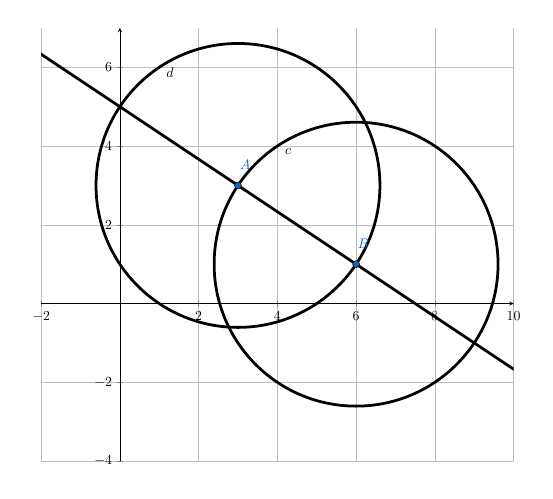
\begin{tikzpicture}[scale = 0.5,line cap=round,line join=round,>=triangle 45,x=1cm,y=1cm]
\begin{axis}[
x=1cm,y=1cm,
axis lines=middle,
ymajorgrids=true,
xmajorgrids=true,
xmin=-2,
xmax=10,
ymin=-4,
ymax=7,
xtick={-8,-6,...,28},
ytick={-12,-10,...,6},]
\clip(-8.5042,-13.986) rectangle (28.667,7.4068);
\draw [line width=2pt,domain=-8.5042:28.667] plot(\x,{(--15-2*\x)/3});
\draw [line width=2pt] (6,1) circle (3.6055512754639896cm);
\draw [line width=2pt] (3,3) circle (3.6055512754639896cm);
\begin{scriptsize}
\draw [fill=rvwvcq] (3,3) circle (2.5pt);
\draw[color=rvwvcq] (3.1844,3.5227) node {$A$};
\draw [fill=rvwvcq] (6,1) circle (2.5pt);
\draw[color=rvwvcq] (6.1852,1.5141) node {$B$};
\draw[color=black] (-2.9382,7.2979) node {$f$};
\draw[color=black] (4.2734,3.8615) node {$c$};
\draw[color=black] (1.2726,5.8701) node {$d$};
\end{scriptsize}
\end{axis}
\end{tikzpicture}
\end{minipage}%
\begin{minipage}{0.5\linewidth}
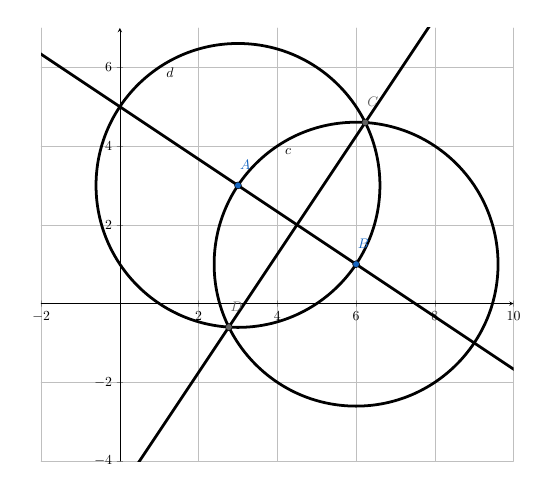
\begin{tikzpicture}[scale=0.5,line cap=round,line join=round,>=triangle 45,x=1cm,y=1cm]
\begin{axis}[
x=1cm,y=1cm,
axis lines=middle,
ymajorgrids=true,
xmajorgrids=true,
xmin=-2,
xmax=10,
ymin=-4,
ymax=7,
xtick={-8,-6,...,28},
ytick={-12,-10,...,6},]
\clip(-8.5042,-13.986) rectangle (28.667,7.4068);
\draw [line width=2pt,domain=-8.5042:28.667] plot(\x,{(--15-2*\x)/3});
\draw [line width=2pt] (6,1) circle (3.6055512754639896cm);
\draw [line width=2pt] (3,3) circle (3.6055512754639896cm);
\draw [line width=2pt,domain=-8.5042:28.667] plot(\x,{(-16.454482671904334--5.196152422706632*\x)/3.464101615137754});
\begin{scriptsize}
\draw [fill=rvwvcq] (3,3) circle (2.5pt);
\draw[color=rvwvcq] (3.1844,3.5227) node {$A$};
\draw [fill=rvwvcq] (6,1) circle (2.5pt);
\draw[color=rvwvcq] (6.1852,1.5141) node {$B$};
\draw[color=black] (-2.9382,7.2979) node {$f$};
\draw[color=black] (4.2734,3.8615) node {$c$};
\draw[color=black] (1.2726,5.8701) node {$d$};
\draw [fill=wrwrwr] (6.232050807568877,4.598076211353316) circle (2.5pt);
\draw[color=wrwrwr] (6.4272,5.1199) node {$C$};
\draw [fill=wrwrwr] (2.767949192431123,-0.5980762113533158) circle (2.5pt);
\draw[color=wrwrwr] (2.9666,-0.0831) node {$D$};
\draw[color=black] (8.218,7.2979) node {$g$};
\end{scriptsize}
\end{axis}
\end{tikzpicture}
\end{minipage}\\%
Lag en vinkelrett linje  på en linje du selv lager ved hjelp av Geogebra.

\question
I denne oppgaven skal vi lære oss å dele en vinkel i to ved hjelp av compass i Geogebra. Dette gjøres på følgende måte:
\begin{enumerate}
\item Tegn to linjer som skjærer hverandre i punktet $A$.
\item Tegn med passer en kurve som skjærer linjene og kall skjæringspunktene på linja for $E$ og $D$.
\item Tegn så med passer to sirkler med lik radius og senter i punktene $E$ og $D$. Trekk deretter en linje fra skje ringspunktet til disse sirklene til punktet $F$
\end{enumerate}
\begin{minipage}{0.5\linewidth}
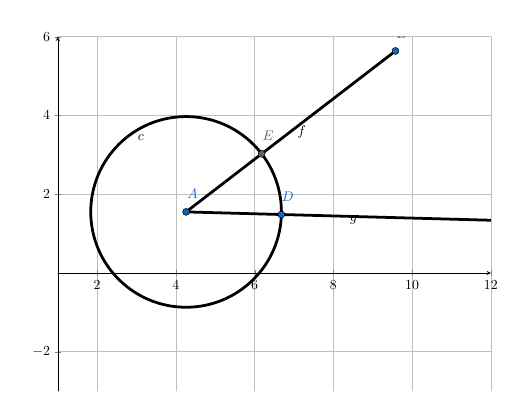
\begin{tikzpicture}[scale = 0.5,line cap=round,line join=round,>=triangle 45,x=1cm,y=1cm]
\begin{axis}[
x=1cm,y=1cm,
axis lines=middle,
ymajorgrids=true,
xmajorgrids=true,
xmin=1,
xmax=12,
ymin=-3,
ymax=6,
xtick={-4,-2,...,26},
ytick={-10,-8,...,6},]
\clip(-4.523082708309361,-11.902528343693854) rectangle (27.514821291549037,6.535952864557977);
\draw [line width=2pt] (4.258139677068495,1.550888374996679)-- (9.576932333294987,5.639058416645275);
\draw [line width=2pt] (4.258139677068495,1.550888374996679)-- (12.643059864531436,1.3214502604143599);
\draw [line width=2pt] (4.258139677068495,1.550888374996679) circle (2.4214765530121887cm);
\begin{scriptsize}
\draw [fill=rvwvcq] (4.258139677068495,1.550888374996679) circle (2.5pt);
\draw[color=rvwvcq] (4.425003760401092,1.9993355989530301) node {$A$};
\draw [fill=rvwvcq] (9.576932333294987,5.639058416645275) circle (2.5pt);
\draw[color=rvwvcq] (9.743796416627584,6.087505640601626) node {$B$};
\draw[color=black] (7.199119145805498,3.58454439061269) node {$f$};
\draw [fill=rvwvcq] (12.643059864531436,1.3214502604143599) circle (2.5pt);
\draw[color=rvwvcq] (12.809923947864032,1.769897484370711) node {$C$};
\draw[color=black] (8.513173802049689,1.3527372760392216) node {$g$};
\draw [fill=rvwvcq] (6.678710206003925,1.4846538580357593) circle (2.5pt);
\draw[color=rvwvcq] (6.8445329687237315,1.9367615677033068) node {$D$};
\draw[color=black] (3.110949104156899,3.438538317696669) node {$c$};
\draw [fill=wrwrwr] (6.178019716676571,3.026560876028767) circle (2.5pt);
\draw[color=wrwrwr] (6.343940718725944,3.4802543385298175) node {$E$};
\end{scriptsize}
\end{axis}
\end{tikzpicture}
\end{minipage}%
\begin{minipage}{0.5\linewidth}
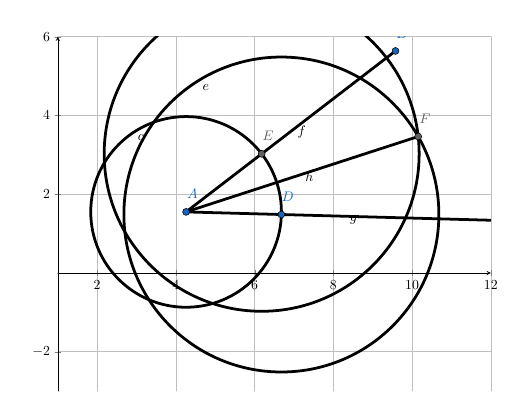
\begin{tikzpicture}[scale = 0.5,line cap=round,line join=round,>=triangle 45,x=1cm,y=1cm]
\begin{axis}[
x=1cm,y=1cm,
axis lines=middle,
ymajorgrids=true,
xmajorgrids=true,
xmin=1,
xmax=12,
ymin=-3,
ymax=6,
xtick={-4,-2,...,26},
ytick={-10,-8,...,6},]
\clip(-4.523082708309361,-11.902528343693854) rectangle (27.514821291549037,6.535952864557977);
\draw [line width=2pt] (4.258139677068495,1.550888374996679)-- (9.576932333294987,5.639058416645275);
\draw [line width=2pt] (4.258139677068495,1.550888374996679)-- (12.643059864531436,1.3214502604143599);
\draw [line width=2pt] (4.258139677068495,1.550888374996679) circle (2.4214765530121887cm);
\draw [line width=2pt] (6.178019716676571,3.026560876028767) circle (4cm);
\draw [line width=2pt] (6.678710206003925,1.4846538580357593) circle (4cm);
\draw [line width=2pt] (4.258139677068495,1.550888374996679)-- (10.153878559127817,3.465362043873891);
\begin{scriptsize}
\draw [fill=rvwvcq] (4.258139677068495,1.550888374996679) circle (2.5pt);
\draw[color=rvwvcq] (4.425003760401092,1.9993355989530301) node {$A$};
\draw [fill=rvwvcq] (9.576932333294987,5.639058416645275) circle (2.5pt);
\draw[color=rvwvcq] (9.743796416627584,6.087505640601626) node {$B$};
\draw[color=black] (7.199119145805498,3.58454439061269) node {$f$};
\draw [fill=rvwvcq] (12.643059864531436,1.3214502604143599) circle (2.5pt);
\draw[color=rvwvcq] (12.809923947864032,1.769897484370711) node {$C$};
\draw[color=black] (8.513173802049689,1.3527372760392216) node {$g$};
\draw [fill=rvwvcq] (6.678710206003925,1.4846538580357593) circle (2.5pt);
\draw[color=rvwvcq] (6.8445329687237315,1.9367615677033068) node {$D$};
\draw[color=black] (3.110949104156899,3.438538317696669) node {$c$};
\draw [fill=wrwrwr] (6.178019716676571,3.026560876028767) circle (2.5pt);
\draw[color=wrwrwr] (6.343940718725944,3.4802543385298175) node {$E$};
\draw[color=black] (4.258139677068495,6.2543697239342215) node {$d$};
\draw[color=black] (4.758731927066283,4.710876953107711) node {$e$};
\draw [fill=wrwrwr] (10.153878559127817,3.465362043873891) circle (2.5pt);
\draw[color=wrwrwr] (10.327820708291668,3.9182725572778816) node {$F$};
\draw[color=black] (7.386841239554668,2.4373538177010943) node {$h$};
\end{scriptsize}
\end{axis}
\end{tikzpicture}
\end{minipage}\\%
\begin{parts}
\part Lag en vinkel ved å tegne to linjer i Geogebra. Del vinkelen mellom dem i to.
\part Konstruer en $45^{\circ}$ vinkel.
\end{parts}
\question
En vinkel på $60^{\circ}$ er konstruert som følger:
\begin{enumerate}
\item Tegn en linje og velg ett punkt $P$ på linja.
\item Bruk passer til å tegn en kurve som skjærer linja i punktet $Q$.
\item Bruk med lik lengde passer til å lage en kurve med sentrum i punktet $Q$.
\item Trekk en linje fra punktet $P$ til skjæringspunktet.
\end{enumerate}
Bruk Geogebra til følgende:
\begin{parts}
  
  \part Konstruer en $60^{\circ}$ vinkel.
  \part Konstruer en $150^{\circ}$ vinkel.
\end{parts}

\question
 Konstruer de følgende vinklene:
\begin{parts}
  \part $135^{\circ}$\\
  \part $225^{\circ}$\\
  \part $120^{\circ}$\\
  \part $150^{\circ}$\\
  \part $210^{\circ}$\\
  \part $245^{\circ}$
\end{parts}

%https://www.mathsteacher.com.au/year8/ch10_geomcons/05_angles/const.htm
\question
Bruk Geogebra til å konstruere ett kvadrat $ABCD$ hvor sidene er av lengde 6.

\question
Bruk Geogebra til å konstruere en trekant $PQR$ der $PQ = 8$, $PR = 7.5$ og $\angle QPR=60^{\circ}$.

\question
Konstuer trekanten $ABC$ der $AB = 8, BC = 6$ og $\angle ABC = 90^{\circ}$.
\begin{parts}
  \part Bruk Geogebra til å måle vinkelen $\angle BAC$ og bruk dette til å regne ut $\angle ACB$.
  \part Bruk Geogebra til å måle $AC$. Bruk dette til å finne omkretsen.
\end{parts}
\question
Konstruer trapeset $PQRS$ der $PQ = 8, PS = 7, QR = 7$ hvor $\angle QPS = 60^{\circ}$ og $\angle PQR =60^{\circ}$. Bruk Geogebra til å finne lengden $RS$. Hva blir da omkretsen av trapeset?
\newpage
\question

\begin{parts}
  \part Konstruer trapeset $DEFG$ der $DE = 6.5, \angle DEF = 90^{\circ}, EF = 5.5, \angle EFG = 90^{\circ}$ og $\angle EDG = 60^{\circ}$.
  \part Regn ut $DGF$ og sjekk svaret med Geogebra.
  \part Regn ut summen av alle vinkelen på innsiden av trapeset.
  \part Bruk Geogebra til å finne $DG,FG$. Hva blir da omkretsen?
\end{parts}

\question
Konstruer trekanten $ABC$ der $AB = 8cm,\angle B = 90^{\circ}$ og $\angle A = 30^{\circ}$.\\
$ABC$ er en del av trapeset $ABCD$ der $\angle CAD = 45^{\circ}$. Konstruer trapeset $ABCD$.

\question
I trekanten $ABC$ er $AB = 7cm, \angle A = 45^{\circ}$ og $\angle B = 60^{\circ}$. Konstruer denne trekanten.\\
$ABC$ er en del av firkanten $ABCD$ der $\angle CAD = 75^{\circ}$ og $AD = 4cm$. Konstruer $ABCD$.

\question
\begin{parts}
  \part Konstruer en likesidet trekant $ABC$ der alle sidene er $6cm$.
  \part Konstruer høyden ned fra $C$ til linja $AB$ i punktet $D$.
  \part Forklar hvorfor $AD = 3cm$.
\end{parts}

\question
I trekanten $ABC$ er $AB=7cm, \angle A=45^{\circ}$ og $B = 60^{\circ}$.\\
$ABC$ er  en del av firkanten $ABCD$ der $\angle ACD = 75^{\circ}$ og $AC=CD$.
\begin{parts}
  \part Konstruer trekanten $ABC$.
  \part Konstruer firkanten $ABCD$.
\end{parts}
\question
\begin{parts}
\part Konstruer en trekant $ABC$ der $AB = 5cm, \angle A = 90^{\circ}$ og $BC = 8cm$.
\part Regn ut $AC$.\\
Trekanten $ABC$ er en del av firkanten $ABCD$ der $\angle ACB = \angle CAD$ og $\angle D = 90^{\circ}$.
\part Konstruer ferdig firkanten $ABCD$.
\part Vis at trekanten $ABC$ er formlik med $DCA$.
\part Regn ut $AD$.
\part Forklar hvorfor firkanten $ABCD$ er ett trapes.
\end{parts}
\end{questions}
\newpage

\section*{Fasit}
\subsection*{1}
Volumet er $253cm^3$, overflaten er $240cm^2$
\subsection*{2}
Volumet er 2.52$l$
\subsection*{3}
$78.63cm$
\subsection*{4}
Volumet er $2548.25cm^3$, overflate $3356.72cm^2$
\subsection*{5}
Sylynderet
\section*{Grubleoppgaver}
{\center \large \bf \underline{Problem 1}}\\
\begin{figure}[h!]
\centering
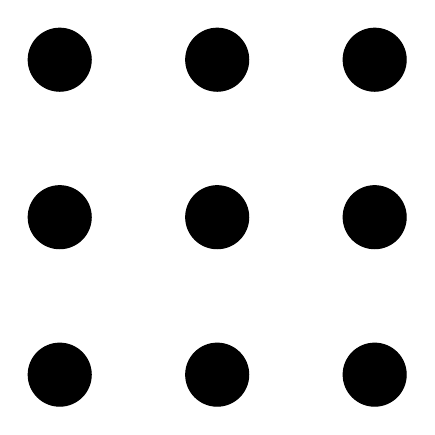
\begin{tikzpicture}[scale=2]
\draw [fill] (0,0) circle [radius=0.2];
\draw [fill] (1,0) circle [radius=0.2];
\draw [fill] (2,0) circle [radius=0.2];

\draw [fill] (0,1) circle [radius=0.2];
\draw [fill] (1,1) circle [radius=0.2];
\draw [fill] (2,1) circle [radius=0.2];

\draw [fill] (0,2) circle [radius=0.2];
\draw [fill] (1,2) circle [radius=0.2];
\draw [fill] (2,2) circle [radius=0.2];
\end{tikzpicture}
\end{figure}
$ $\\

Sett blyanten ned ett sted og tegn 4 rette linjer uten å ta blyanten opp fra arket. Disse linjene skal innom alle de 9 prikkene.


\newpage
{\center \large \bf \underline{Problem 2}}\\
Diagrammet viser en epleåker. Gartneren startet på stjerna og gikk innom alle feltene selv de med og uten ett tre. Han gikk aldri på det samme feltet to ganger og sluttet på stjerna. Kan du finne ut hvor gartneren gikk?
\begin{figure}[h!]
\centering
\begin{tikzpicture}
\draw[step=1cm,gray,very thin] (0,0) grid (8,8);
% 8th row
\node at (8-0.5,8-0.5) {\faStar};
\node at (7-0.5,8-0.5) {\Huge $\cdot$};
\node at (5-0.5,8-0.5) {\Huge $\cdot$};
\draw [fill=gray] (3,8) rectangle (2,7);
\node at (1-0.5,8-0.5) {\Huge $\cdot$};
% 7th row
\node at (8-0.5,7-0.5) {\Huge $\cdot$};
\node at (6-0.5,7-0.5) {\Huge $\cdot$};
\node at (4-0.5,7-0.5) {\Huge $\cdot$};
\draw [fill=gray] (3,7) rectangle (2,6);
\node at (2-0.5,7-0.5) {\Huge $\cdot$};
% 6th row
\node at (7-0.5,6-0.5) {\Huge $\cdot$};
\node at (5-0.5,6-0.5) {\Huge $\cdot$};
\node at (3-0.5,6-0.5) {\Huge $\cdot$};
\node at (1-0.5,6-0.5) {\Huge $\cdot$};
% 5th row
\node at (8-0.5,5-0.5) {\Huge $\cdot$};
\node at (6-0.5,5-0.5) {\Huge $\cdot$};
\draw [fill=gray] (4,5) rectangle (3,4);
\node at (2-0.5,5-0.5) {\Huge $\cdot$};
% 4th row
\node at (7-0.5,4-0.5) {\Huge $\cdot$};
\node at (5-0.5,4-0.5) {\Huge $\cdot$};
\draw [fill=gray] (4,4) rectangle (3,3);
\node at (3-0.5,4-0.5) {\Huge $\cdot$};
\node at (1-0.5,4-0.5) {\Huge $\cdot$};
% 3rd row
\node at (8-0.5,3-0.5) {\Huge $\cdot$};
\node at (6-0.5,3-0.5) {\Huge $\cdot$};
\node at (4-0.5,3-0.5) {\Huge $\cdot$};
\node at (2-0.5,3-0.5) {\Huge $\cdot$};
% 2nd row
\node at (7-0.5,2-0.5) {\Huge $\cdot$};
\draw [fill=gray] (5,2) rectangle (4,1);
\node at (3-0.5,2-0.5) {\Huge $\cdot$};
\node at (1-0.5,2-0.5) {\Huge $\cdot$};
% 1st  row
\draw [fill=gray] (5,1) rectangle (4,0);
\node at (8-0.5,1-0.5) {\Huge $\cdot$};
\node at (6-0.5,1-0.5) {\Huge $\cdot$};
\node at (4-0.5,1-0.5) {\Huge $\cdot$};
\node at (2-0.5,1-0.5) {\Huge $\cdot$};
\end{tikzpicture}
\end{figure}
{\center \large \bf \underline{Problem 3}}\\
Jeg har plassert tallene 1,2 og 3 langs hjørnene i en trekant. Skriv tallene 4,5,6,7,8 og 9 langs sidene på trekanten sånn at summen langs sidene blir 17.
\begin{figure}[h!]
  \centering
  \begin{tikzpicture}
    \draw (0,0) node[anchor = north east] {1} -- (5,0) node[anchor = north west]{3};
    \draw (0,0) -- (2.5,5.2) node[anchor = south] {2};
    \draw (2.5,5.2) -- (5,0);
  \end{tikzpicture}
\end{figure}


\end{document}






% Perp line
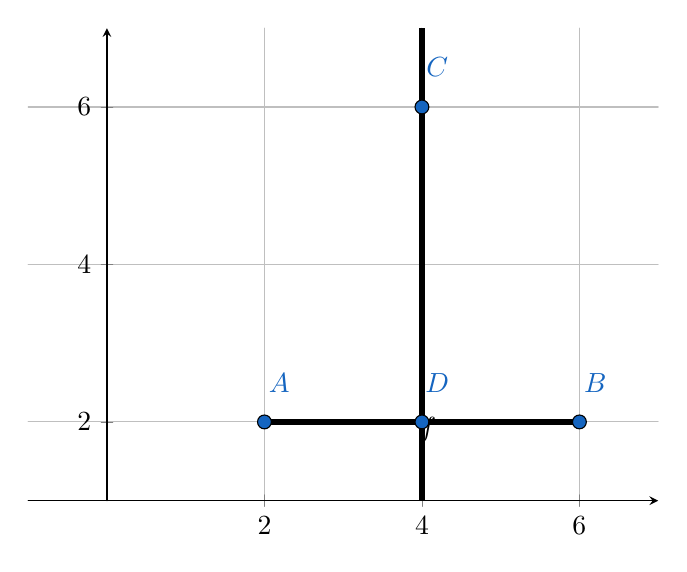
\begin{tikzpicture}[line cap=round,line join=round,>=triangle 45,x=1cm,y=1cm]
\begin{axis}[
x=1cm,y=1cm,
axis lines=middle,
ymajorgrids=true,
xmajorgrids=true,
xmin=-1,
xmax=7,
ymin=1,
ymax=7,
xtick={-16,-14,...,18},
ytick={-12,-10,...,6},]
\clip(-16.91341019955654,-13.520017738359199) rectangle (19.35117516629712,7.351006651884704);
\draw [line width=2pt] (2,2)-- (6,2);
\draw [line width=2pt] (4,-13.520017738359199) -- (4,7.351006651884704);
\begin{scriptsize}
\draw [fill=rvwvcq] (2,2) circle (2.5pt);
\draw[color=rvwvcq] (2.1868824833702907,2.4992017738359236) node {$A$};
\draw [fill=rvwvcq] (6,2) circle (2.5pt);
\draw[color=rvwvcq] (6.200541019955657,2.4992017738359236) node {$B$};
\draw [fill=rvwvcq] (4,6) circle (2.5pt);
\draw[color=rvwvcq] (4.193711751662974,6.512860310421289) node {$C$};
\draw[color=black] (4.075662971175169,1.9089578713968995) node {$f$};
\draw [fill=rvwvcq] (4,2) circle (2.5pt);
\draw[color=rvwvcq] (4.193711751662974,2.4992017738359236) node {$D$};
\draw[color=black] (3.697906873614193,7.244762749445679) node {$g$};
\end{scriptsize}
\end{axis}
\end{tikzpicture}

